\def\thetitle{Homework 1}
\pagebreak

\begin{center}
    
\includegraphics[height=0.075\textheight]{images/LogoYachay.pdf} 
    \hspace{0.1\linewidth}
    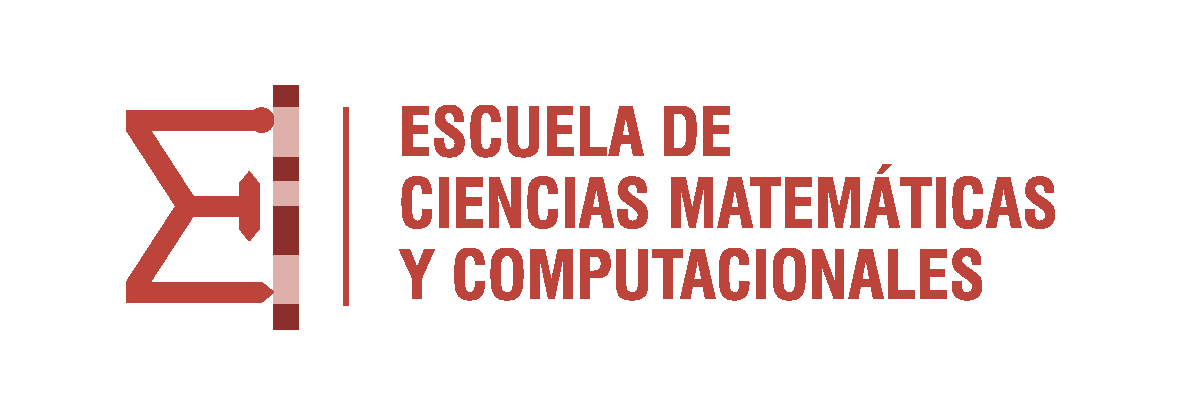
\includegraphics[height=0.075\textheight]{images/LogoECMC.pdf}
\end{center}

% \phantomsection\pdfbookmark{\currfilebase}{\currfilebase}

\begin{center}
    {\LARGE
    Abstract Algebra 2024--I\\
    % Teaching Assistant
    \vspace{0.25cm}
    \textbf{\thetitle{}}}

    % \emph{I hear, I forget;    I see, I remember;     I do, I understand.}
    
    Pablo Rosero \& Christian Chávez
    
    % \today

    September 11, 2023
\end{center}

% \setcounter{problem}{0}


\begin{questions}

\question
  For each of the following pairs of integers \(a\) and \(b\), determine their greatest common divisor, their least common multiple, and write their greatest common divisor in the form \(a x+b y\) for some integers \(x\) and \(y\).
  \begin{enumerate}[label=(\alph*)]
    \item \(a=792, b=275\)
    \item \(a=507885, b=60808\)
  \end{enumerate} 

\begin{solution}
    \begin{enumerate}[label=(\alph*)]
        \item \(\gcd(a,b) = 11\), \(\lcm(a,b) = 19800\), \(\gcd(a,b)= 8a - 23b\)
        \item \(\gcd(a,b) = 691\), \(\lcm(a,b) = 44693880\), \(\gcd(a,b)= -17a +142b\)
    \end{enumerate}
\end{solution}


\question
    Prove that if \({n}\) is composite then there are integers \(a\) and \(b\) such that \(n\) divides \(a b\) but \(n\) does not divide either \(a\) or \(b\).

\begin{solution}
    Let \(n\) be composite. By definition we have \(n=a b\) for some integers \(a\) and \(b\) with \(a, b \neq \pm 1, \pm n\). Clearly \(n \mid a b\). Now suppose by way of contradiction that \(n \mid a\). Then we have \(k n=a\) for some integer \(k\). Now \(k b a=a\), so \((k b-1) a=0\), so \(k b=1\). Thus \(b= \pm 1\), a contradiction. Hence,  \(n\) does not divide \(a\). Similarly, \(n\) does not divide \(b\).
\end{solution}

\question
    If \(p\) is a prime prove that there do not exist nonzero integers \(a\) and \(b\) such that \(a^2=p b^2\) (i.e., \(\sqrt{p}\) is not a rational number).


% Dummit p. 11 ------------------------

\question
    Write down explicitly all the elements in the residue classes of \(\mathbb{Z} / 18 \mathbb{Z}\).




\begin{solution}
    
\end{solution}

\question
    Prove that if \(a=a_n 10^n+a_{n-1} 10^{n-1}+\cdots+a_1 10+a_0\) is any positive integer then \(a \equiv a_n+a_{n-1}+\cdots+a_1+a_0(\bmod 9)(\) note that this is the usual arithmetic rule that the remainder after division by 9 is the same as the sum of the decimal digits mod \(9-\) in particular an integer is divisible by 9 if and only if the sum of its digits is divisible by 9 ) [note that \(10 \equiv 1(\bmod 9)\) ].


\begin{solution}
    
\end{solution}

\question
    Compute the remainder when \(37^{100}\) is divided by 29.


\begin{solution}
    
\end{solution}

\question
    Prove that the squares of the elements in \(\mathbb{Z} / 4 \mathbb{Z}\) are just \(\overline{0}\) and \(\overline{1}\).


\begin{solution}
    
\end{solution}

\question
    Prove for any integers \(a\) and \(b\) that \(a^2+b^2\) never leaves a remainder of 3 when divided by 4 (use the previous exercise).


\begin{solution}
    
\end{solution}


\question
    Prove that the equation \(a^2+b^2=3 c^2\) has no solutions in nonzero integers \(a, b\) and \(c\). [Consider the equation mod 4 as in the previous two exercises and show that \(a, b\) and \(c\) would all have to be divisible by 2 . Then each of \(a^2, b^2\) and \(c^2\) has a factor of 4 and by dividing through by 4 show that there would be a smaller set of solutions to the original equation. Iterate to reach a contradiction.]


\begin{solution}
    
\end{solution}


\question
    Prove that if \(\bar{a}, \bar{b} \in(\mathbb{Z} / n \mathbb{Z})^{\times}\), then \(\bar{a} \cdot \bar{b} \in(\mathbb{Z} / n \mathbb{Z})^{\times}\).


\begin{solution}
    
\end{solution}


\question
    Let \(n \in \mathbb{Z}, n>1\), and let \(a \in \mathbb{Z}\) with \(1 \leq a \leq n\). Prove if \(a\) and \(n\) are not relatively prime, there exists an integer \(b\) with \(1 \leq b<n\) such that \(a b \equiv 0(\bmod n)\) and deduce that there cannot be an integer \(c\) such that \(a c \equiv 1(\bmod n)\).


\begin{solution}
    
\end{solution}


\question
    Let \(n \in \mathbb{Z}, n>1\), and let \(a \in \mathbb{Z}\) with \(1 \leq a \leq n\). Prove that if \(a\) and \(n\) are relatively prime then there is an integer \(c\) such that \(a c \equiv 1(\bmod n)\), [use the fact that the g.c.d. of two integers is a \(\mathbb{Z}\)-linear combination of the integers].



\begin{solution}
    
\end{solution}


\question
    Conclude from the previous two exercises that \((\mathbb{Z} / n \mathbb{Z})^{\times}\)is the set of elements \(\bar{a}\) of \(\mathbb{Z} / n \mathbb{Z}\) with \((a, n)=1\) and hence prove Proposition 4 . Verify this directly in the case \(n=12\).



% Page 5 from [book] ----------------------------------

\begin{solution}
    
\end{solution}


\question
    \begin{enumerate}[label=(\alph*)]
        \item Prove that if \(n\) is squarefree (i.e., \(n>1\) and \(n\) is not divisible by the square of any prime), then \(\sqrt{n}\) is irrational.
        \item Prove that \(\sqrt[3]{2}\) is irrational.
    \end{enumerate}


\begin{solution}
    
\end{solution}


\question
    If \(d=(a, b)\), prove that \(a / d\) and \(b / d\) are relatively prime.


\begin{solution}
    
\end{solution}


\question
    Prove that if \((r, m)=1=\left(r^{\prime}, m\right)\), then \(\left(r r^{\prime}, m\right)=1\).


\begin{solution}
    
\end{solution}


\question
    Assume that \(d=s a+t b\) is a linear combination of integers \(a\) and \(b\). Find infi nitely many pairs of integers \(\left(s_k, t_k\right)\) with
\[
d=s_k a+t_k b
\]


\begin{solution}
    
\end{solution}


\question
    If \(a\) and \(b\) are relatively prime and if each divides an integer \(n\), then their product \(a b\) also divides \(n\).


\begin{solution}
    
\end{solution}


\question
    If \(a>0\), prove that \(a(b, c)=(a b, a c)\). [One must assume that \(a>0\) lest \(a(b, c)\) be negative.]


\begin{solution}
    
\end{solution}


\question
     A Pythagorean triple is a triple \((a, b, c)\) of positive integers for which
\[
a^2+b^2=c^2
\]
it is called primitive if the \(\operatorname{gcd}(a, b, c)=1\).
\begin{enumerate}[label=(\alph*)]
    \item Consider a complex number \(z=q+i p\), where \(q>p\) are positive integers. Prove that
\[
\left(q^2-p^2, 2 q p, q^2+p^2\right)
\]
is a Pythagorean triple by showing that \(\left|z^2\right|=|z|^2\). [One can prove that every primitive Pythagorean triple \((a, b, c)\) is of this type.]
\item Show that the Pythagorean triple \((9,12,15)\) (which is not primitive) is not of the type given in part (i).

\end{enumerate}


\begin{solution}
    
\end{solution}


\question
    Let \(X=\left\{x_1, \ldots, x_m\right\}\) and \(Y=\left\{y_1, \ldots, y_n\right\}\) be fi nite sets, where the \(x_i\) are distinct and the \(y_j\) are distinct. Show that there is a bijection \(f: X \rightarrow Y\) if and only if \(|X|=|Y|\); that is, \(m=n\).


\begin{solution}
    
\end{solution}


\question[Pigeonhole Principle]
    If \(X\) and \(Y\) are fi nite sets with the same number of elements, show that the following conditions are equivalent for a function \(f: X \rightarrow Y\).
    \begin{enumerate}[label=(\alph*)]
        \item \(f\) is injective;
        \item \(f\) is bijective;
        \item \(f\) is surjective.
    \end{enumerate}



\begin{solution}
    
\end{solution}


\question
    \begin{enumerate}[label=(\alph*)]
        \item Let \(f: X \rightarrow Y\) be a function, and let \(\left\{S_i: i \in I\right\}\) be a family of subsets of \(X\). Prove that
\[
f\left(\bigcup_{i \in I} S_i\right)=\bigcup_{i \in I} f\left(S_i\right)
\]

        \item If \(S_1\) and \(S_2\) are subsets of a set \(X\), and if \(f: X \rightarrow Y\) is a function, prove that \(f\left(S_1 \cap S_2\right) \subseteq f\left(S_1\right) \cap f\left(S_2\right)\). Give an example in which \(f\left(S_1 \cap S_2\right) \neq f\left(S_1\right) \cap f\left(S_2\right)\).
        
        \item If \(S_1\) and \(S_2\) are subsets of a set \(X\), and if \(f: X \rightarrow Y\) is an injection, prove that \(f\left(S_1 \cap S_2\right)=f\left(S_1\right) \cap f\left(S_2\right)\).
    \end{enumerate}


\begin{solution}
    
\end{solution}


\question
    Let \(f: X \rightarrow Y\) be a function.
    \begin{enumerate}[label=(\alph*)]
        \item If \(B_i \subseteq Y\) is a family of subsets of \(Y\), prove that
\[
f^{-1}\left(\bigcup_i B_i\right)=\bigcup_i f^{-1}\left(B_i\right) \text { and } f^{-1}\left(\bigcap_i B_i\right)=\bigcap_i f^{-1}\left(B_i\right) \text {. }
\]
        \item If \(B \subseteq Y\), prove that \(f^{-1}\left(B^{\prime}\right)=f^{-1}(B)^{\prime}\), where \(B^{\prime}\) denotes the complement of \(B\).
    \end{enumerate}



\begin{solution}
    
\end{solution}


\question
    Let \(f: X \rightarrow Y\) be a function. Defi ne a relation on \(X\) by \(x \equiv x^{\prime}\) if \(f(x)=f\left(x^{\prime}\right)\). Prove that \(\equiv\) is an equivalence relation. If \(x \in X\) and \(f(x)=y\), the equivalence class \([x]\) is usually denoted by \(f^{-1}(y)\), the inverse image of \(\{y\}\).

\begin{solution}
    
\end{solution}
\end{questions}